\section{Introduction} \label{sec:2.1}

% ! In the first chapter, you should explain about the fuzzers, how they cover the implementation bugs and how their performances are.
% ! A vulnerability is a reproducable state of a program's execution, that the program fails to execute as expected. 

%? What is fuzzing
Fuzzing (short for fuzz testing) is a tool for \say{finding implementation bugs using malformed/semi-malformed data injection in an automated fashion}
% TODO: requires citation?
. Since the late '80s, fuzz testing has proved to be a powerful tool for finding errors in a program. For instance, American Fuzzy Lopper (AFL) has found more than a total of 330 vulnerabilities from 2013 to 2017 in more than 70 different programs \cite{afl_cve}. The research on fuzz testing has found its place in software security testing. Liang et al. \cite{liang2018fuzzing} illustrates the growth of the primary studies from the following publishers: \textit{ACM digital library}, \textit{Elsevier ScienceDirect}, \textit{IEEEXplore digital library}, \textit{Springer online library}, \textit{Wiley InterScience}, \textit{USENIX}, and \textit{Semantic scholar}. The queries for the literature reviews are "fuzz testing", "fuzzing", "fuzzer", "random testing", or "swarm testing" as the keywords of the titles. Figure \ref{fig:fuzz_articles} presents the results of the mentioned study.

\begin{figure}[!t]
    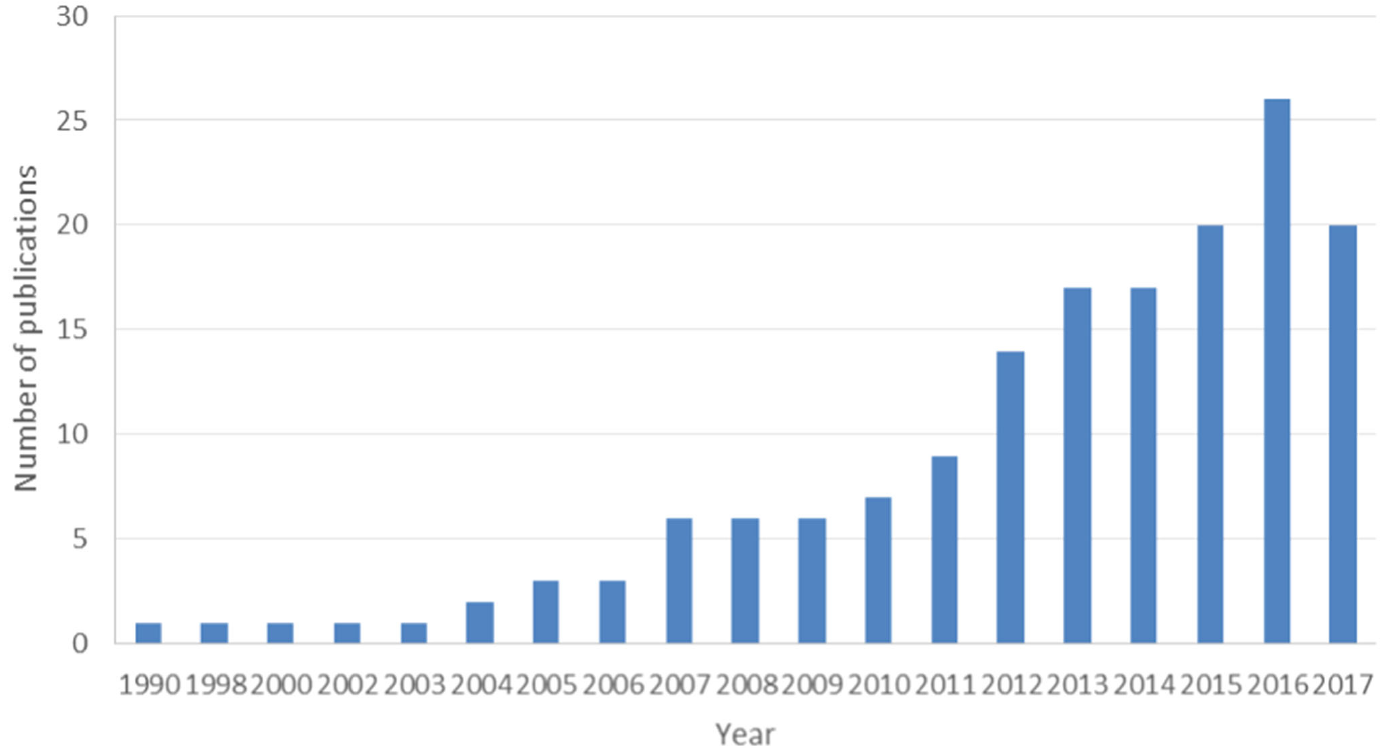
\includegraphics[width=\textwidth]{Chapter2/fuzz_articles.png}
    \centering
    \caption{Fuzzing papers published between January 1st, 1990 and June 30 2017. \cite{liang2018fuzzing}}
    \label{fig:fuzz_articles}
\end{figure}

%? How does a fuzzer start
A \textit{run} is a sequence of instructions that connects the start and termination of a program. A successful run (execution) behaves as the program is intended to run. An exception is a signal that is thrown, indicating an unexpected behavior. If the exception is not caught before the program's termination, the operating system receives an unfinished task with the exception's descriptions. From the OS's perspective, the program has crashed and could not finish its execution properly. A software vulnerability is an unexpected state of the program that is failed to be handled. Different states of a program occur by different inputs that a program takes. The inputs such as \textit{environment variables}, \textit{file paths}, or other program's \textit{arguments} are mainly selected to search for the vulnerabilities. 

% ? How does the fuzzing's iterations continue
Fuzz testing is the repetitive executions of a target program with different inputs. Fuzz testing takes two main actions in the fuzzing procedure: the fuzzer \textit{generates test cases} for the target program, and each generated (fuzzed) test case is then passed to the program for \textit{execution}. A fuzzer gathers information out of each execution. A \textit{whitebox} fuzzer has access to the source code of the target program. \textit{Analyzing the source code}, \textit{monitoring the execution}, and \textit{validating the returned value of execution}, are of the capabilities of a whitebox fuzzer. Oppositely, a \textit{blackbox} fuzzer does not have any access to the source code, cannot analyze the execution and does not check the result of the execution. Instead, a blackbox fuzzer focuses on executing more instances of the program blindly. Fuzzers with at least one property from each of the whitebox and blackbox fuzzers are in the category of \textit{greybox} fuzzers.

%? Generate test cases
The common strategies for fuzzing new test cases include \textit{genetic algorithms}, \textit{coverage-based (coverage-guided) strategies}, \textit{performance fuzzing}, \textit{symbolic execution}, \textit{taint-based analysis}, etc. Genetic algorithms (GA) are \textit{evolutionary algorithms} for generating solutions to \textit{search} and \textit{optimization problems}. GA has a population of solutions that their evaluations affect their survivability for the next generation. Inspired by the biological operations, GA processes the selected (survived) population and applies \textit{mutations} and other modifications on them, resulting in a new generation of the population \cite{banzhaf1998genetic, whitley1994genetic}. Coverage-guided strategy is a genetic algorithm that utilizes \textit{concrete analysis} of the \textit{execution-path} of a program. A concrete analysis investigates the runtime information of an executive program, and the graph of the executed instructions (execution-path) can be collected through this analysis. Symbolic executions determine the constraints that change the execution-paths \cite{bohme2017coverage}. Performance fuzzing is a coverage-based technique that generates \textit{pathological inputs}. \say{Pathological inputs are those inputs which exhibit worst-case algorithmic complexity in different components of the program} \cite{lemieux2018perffuzz}. A taint-based analysis of a program tracks back the variables that cause a state of the executing program. This approach can detect vulnerabilities with no false positives \cite{newsome2005dynamic}. 

%? Execution 
American Fuzzy Lopper (AFL) \cite{afl_git} is a coverage-based greybox fuzzer, that is originally considering the number of times each \textit{basic block} of execution is visited. Each basic block is a sequence of instructions with no branches except the entry (jump in) and exit (jump out) of the sequence. AFL is published with two default tools for collecting the runtime information: \textit{LLVM} \cite{llvm} and \textit{QEMU} \cite{bellard2005qemu}. \say{The LLVM Project is a collection of modular and reusable compiler and toolchain technologies. Despite its name, LLVM has little to do with traditional virtual machines. The name "LLVM" itself is not an acronym; it is the full name of the project.} AFL acts as a \textbf{whitebox} fuzzer in \textit{llvm-mode}. In \textbf{llvm-mode}, AFL provides the recipe for compiling the target program with coverage information. The resulting compiler adds \textit{static instrumentations} (\textbf{SI}) to the program. Instrumentation is the process of injecting logging instructions into the program, and SI refers to the instrumentations applied on a binary before execution. The added instructions store the code coverage and AFL can use them in Fuzzing. QEMU (Quick EMUlator) is an open-source emulator and virtualizer that helps AFL with \textit{dynamic instrumentation} (\textbf{DI}). In DI, the instructions are inserted in runtime, and an emulator such as QEMU helps AFL with discovering the code coverage \cite{afl_qemu}. \textit{DynamoRIO} \cite{dynamorio}, \textit{Frida} \cite{frida}, and \textit{PIN} \cite{pin} are some other examples of pioneer DI tools.

%? Wrap it up
In this chapter, we begin with reviewing the previous works that lead to this thesis \ref{sec:2-lit}. Next, we describe the implementation of AFL and its llvm-mode in \ref{sec:2.3}. We wrap up this chapter with conclusions.
